\documentclass{article}

\usepackage{graphicx} % Required for the inclusion of images
\usepackage{natbib} % Required to change bibliography style to APA
\usepackage{amsmath} % Required for some math elements 


\usepackage{amssymb}
\usepackage{amsmath}
\usepackage{float}

\usepackage{caption}

\usepackage{enumitem}
\usepackage{booktabs}

\usepackage{multirow}

\usepackage{amsmath}

\usepackage{subcaption}
\captionsetup{compatibility=false}

\floatstyle{plaintop}
\restylefloat{table}

%%%%%%%%%% <GIF> %%%%%%%%%%%
\usepackage{epstopdf}

\epstopdfDeclareGraphicsRule{.gif}{png}{.png}{convert gif:#1 png:\OutputFile}
\AppendGraphicsExtensions{.gif}
%%%%%%%%%% </GIF> %%%%%%%%%%%

\setlength\parindent{0pt} % Removes all indentation from paragraphs

\renewcommand{\labelenumi}{\alph{enumi}.} % Make numbering in the enumerate environment by letter rather than number (e.g. section 6)

%\usepackage{times} % Uncomment to use the Times New Roman font

%----------------------------------------------------------------------------------------
%	DOCUMENT INFORMATION
%----------------------------------------------------------------------------------------

\title{Biometrics \\ Laboratory Report} % Title

\author{Jakub \textsc{Ciecierski}} % Author name

\date{\today} % Date for the report

\begin{document}

\maketitle % Insert the title, author and date

\begin{center}
\begin{tabular}{l r}
Date Performed: & October 30, 2015 \\ % Date the experiment was performed
\end{tabular}

\vspace{60pt}

\includegraphics[width=80mm]{res/mini.PNG} \\
\end{center}

% If you wish to include an abstract, uncomment the lines below
% \begin{abstract}
% Abstract text
% \end{abstract}

\newpage

	\tableofcontents
	
\newpage

%----------------------------------------------------------------------------------------
\section{KMM}

%----------------------------------------------------------------------------------------
%----------------------------------------------------------------------------------------
\subsection{Algorithm}

%----------------------------------------------------------------------------------------
%----------------------------------------------------------------------------------------
%----------------------------------------------------------------------------------------
\subsubsection{KMM - Main}
KMM works as follows

\begin{enumerate}
	\item Convert input image into normalized and binary image
	\item Initialize a Bit Map based on the image. Corresponding elements of black pixels have value 1, white pixels have 0.
	
	\item Choose Sticking Pixel To background.
	\begin{enumerate}
		\item Pixels that stick with background directly (South, North, East, West) are given value 2. 
		\item Pixels that stick with background by corners (South-East, South-West, North-East, North-West) are given value 3.
	\end{enumerate}
	
	\item Select Pixel for deletion by giving them values 4. Consider a $3 \times 3$ Matrix of weights (see Implementation for details). For each Pixel do:

	\begin{enumerate}
		\item Let the current Pixel be the anchor point of Weight Matrix which is placed in the middle of that Matrix. For all neighbours in that area, compute the sum of corresponding weights.
		\item Refer to Deletion Array to see if Pixel with given sum of weights should be deleted or not. If it is in Deletion Array, set value of that Pixel to 4
	\end{enumerate}
	
	\item Remove certain Pixels without Loss of Connectivity
	\begin{enumerate}
		\item Remove Pixels with value 2 without $LoC$.
		\item Remove Pixels with value 3 without $LoC$.
	\end{enumerate}
	
	\item Repeat $a.$ through $e.$ until no further changes have been made
\end{enumerate}

%----------------------------------------------------------------------------------------
%----------------------------------------------------------------------------------------
%----------------------------------------------------------------------------------------
\subsubsection{KMM - Loss of Connectivity}

The algorithm for checking if pixels can be removed without Loss of Connectivity is looks as follows:

\begin{enumerate}
	\item For input Pixel create its local 8-point neighbourhood
	\item Initialize each element in the neighbourhood:
	\begin{enumerate}
		\item If value of corresponding element in Bit Map is 0 then set value to 0
		\item Otherwise set it to 1.
	\end{enumerate}
	\item The element of neighbourhood corresponding to input Pixel is given value 0. As to imitate the situation where this pixel was removed.
	
	\item If the neighbourhood is connected then input Pixel can be removed
\end{enumerate}

%----------------------------------------------------------------------------------------
%----------------------------------------------------------------------------------------
%----------------------------------------------------------------------------------------
\subsubsection{KMM - Neighbourhood Connectivity}

The algorithm for checking if the given neighbourhood is connected

\begin{enumerate}
	\item Choose one of the elements with value 1 as source. If no such element exists, stop the algorithm

	\item Consider a Reachability Flags. 0 if corresponding node is unreachable, 1 if it is reachable.
		\begin{enumerate}
		\item Initialize flags for all nodes to 0. Initialize flag for source node to 1.
		\end{enumerate}
	\item Consider Current Nodes queue - holds nodes to be checked.
	\begin{enumerate}
		\item Insert source node to queue.
	\end{enumerate}
	
	\item Dequeue the Current Node.
			\begin{enumerate}
		\item For all other nodes that are connected to Current Node
		\begin{enumerate}
			\item If this node has Reachability Flag 0. Change flag value to 1 and add to Current Nodes queue.
		\end{enumerate}
		\item Repeat util the queue is empty
		\end{enumerate}

	\item If all Nodes are reachable from source. Then neighbourhood is connected.
	
\end{enumerate}
\subsection{Implementation}

The implementation details of KMM algorithm are presented.
Figure~\ref{fig:kmm_header} shows the header of the KMM class. The Sticky Neighbours array defines which value should the pixels sticking to border pixels take. The Binary Weights array is used as template to compute the weight in the thinning phase.

The figure~\ref{fig:kmm_deletion} shows the Deletion array used determine whether a pixel with given sum of weights should be deleted or not.

The main iterative procedure is presented in figure~\ref{fig:kmm_compute}. The $bitMap$ is used to represent the image.

The step 0 - the filter step - turns the image into a binary one. The step 1. is simply an initialization of the bit map, where black pixels get value 1, and white pixels get value 0. The $updateImageWithBitMap$ simply updates the image pixels based on the bit map values. These methods are presented in figure~\ref{fig:kmm_filter}.

Choosing Pixels sticking to background phase is presented in figure~\ref{fig:kmm_stick_bg}. The $StickyNeighbours$ Look Up table is used to determine which value should the corresponding pixel get, sticking directly or sticking by the corner.

Further, step 3, chooses and deletes pixels based on the binary weights. $BinaryWeights$ array is used to calculate the sum of corresponding neighbours. Then the $Deletion Array$ checks whether a tested Pixel should be deleted. This is presented in figure~\ref{fig:kmm_binary_weights}.

The step 4. removes the pixels without loss of connectivity. The main method of that procedure is shown in figure~\ref{fig:kmm_conn_main}. The idea is to create a neighbourhood for each pixel that we are considering to delete. The neighbourhood is initialized based on the corresponding pixels in the image. The target Pixel is removed from the neighbourhood by setting the corresponding element to Background value. Source pixel representing a interior point is then chosen. The $isConnectedToAll$ method will check whether the source is connected to all other interior points in the neighbourhood. This method is presented in figure~\ref{fig:kmm_conn_is_conn}.
The idea is to compute whether all interior points in the neighbourhood are connected to each other after temporally removing the tested Pixel. If this is true, then this Pixel can be safely removed.

Finally a few utility methods used through out the algorithm are presented in figure~\ref{fig:kmm_util}.

%%%%
%
% Header
%
%%%%
\begin{figure}[H]
\centering

  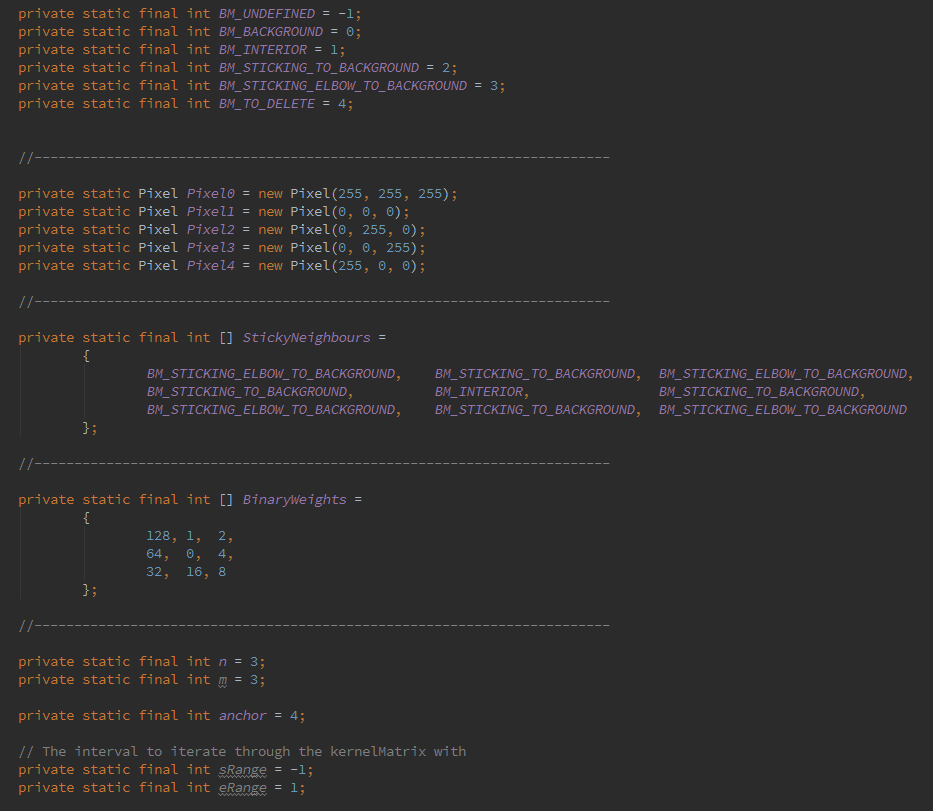
\includegraphics[width=0.9\linewidth]{res/kmm/class_header.png}

\caption{Header of KMM Class}
\label{fig:kmm_header}
\end{figure}



%%%%
%
% Deletion Array
%
%%%%
\begin{figure}[H]
\centering

  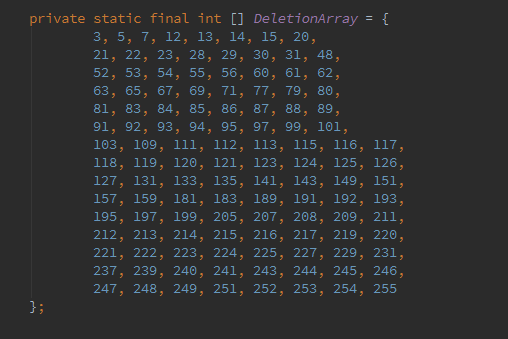
\includegraphics[width=0.9\linewidth]{res/kmm/deletion.png}

\caption{Deletion Array}
\label{fig:kmm_deletion}
\end{figure}





%%%%
%
% Compute
%
%%%%
\begin{figure}[H]
\centering

  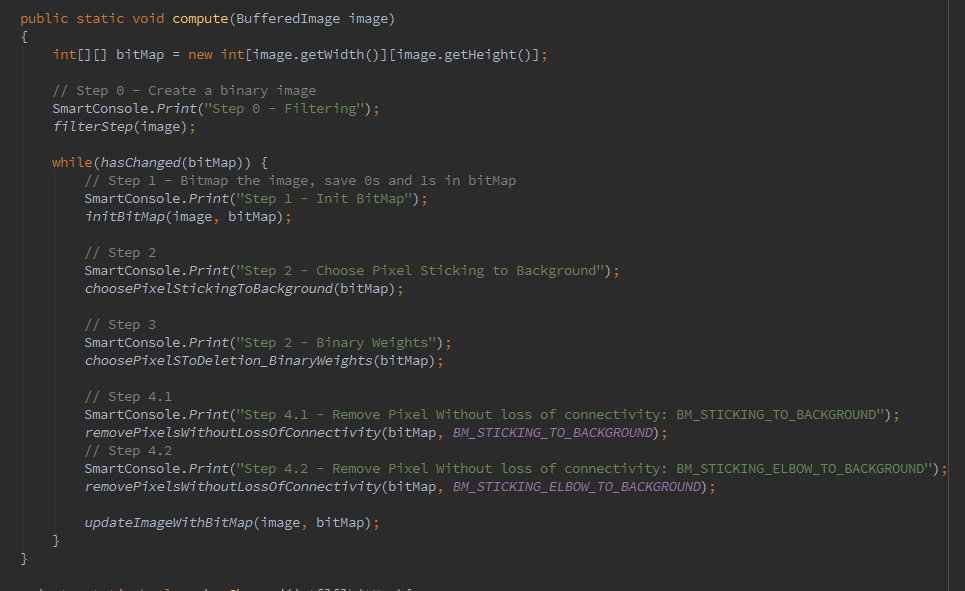
\includegraphics[width=0.9\linewidth]{res/kmm/compute.png}

\caption{Main Compute method}
\label{fig:kmm_compute}
\end{figure}


%%%%
%
% Filter
%
%%%%
\begin{figure}[H]
\centering

  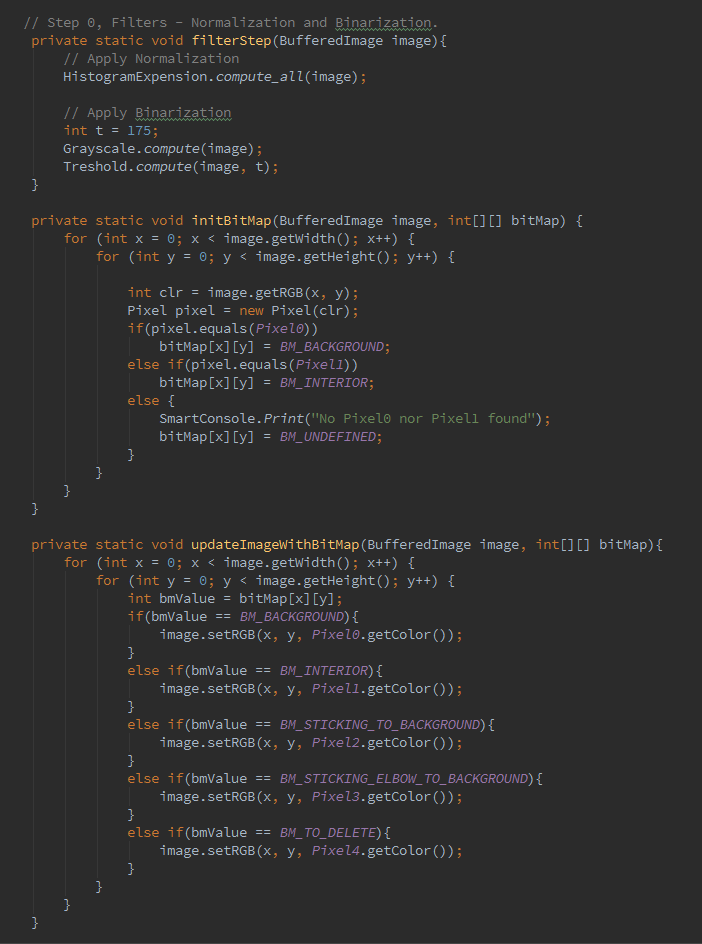
\includegraphics[width=0.9\linewidth]{res/kmm/filter_bitmap.png}

\caption{Filter and BitMap stage}
\label{fig:kmm_filter}
\end{figure}


%%%%
%
% Sticking to Background
%
%%%%
\begin{figure}[H]
\centering

  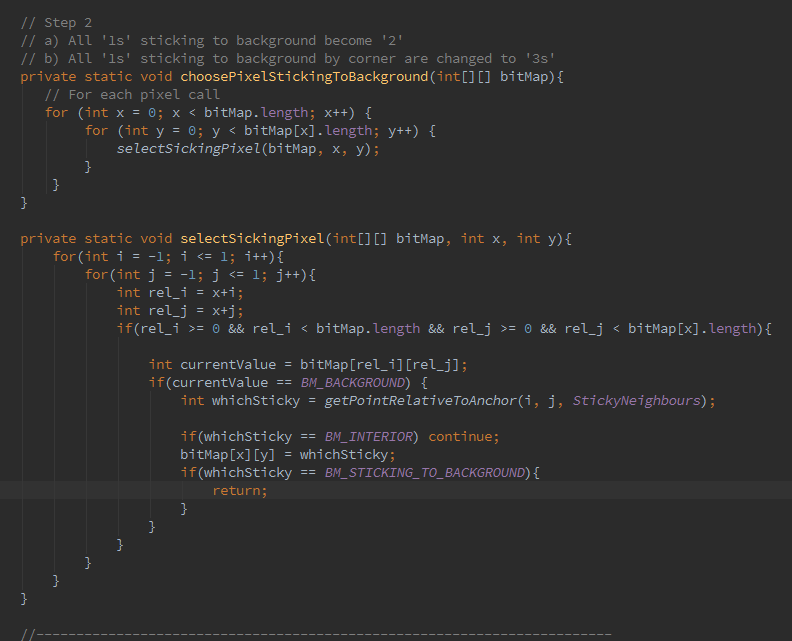
\includegraphics[width=0.9\linewidth]{res/kmm/stick_bg.png}

\caption{Choosing Pixels Sticking to Background}
\label{fig:kmm_stick_bg}
\end{figure}


%%%%
%
% Binary Weights
%
%%%%
\begin{figure}[H]
\centering

  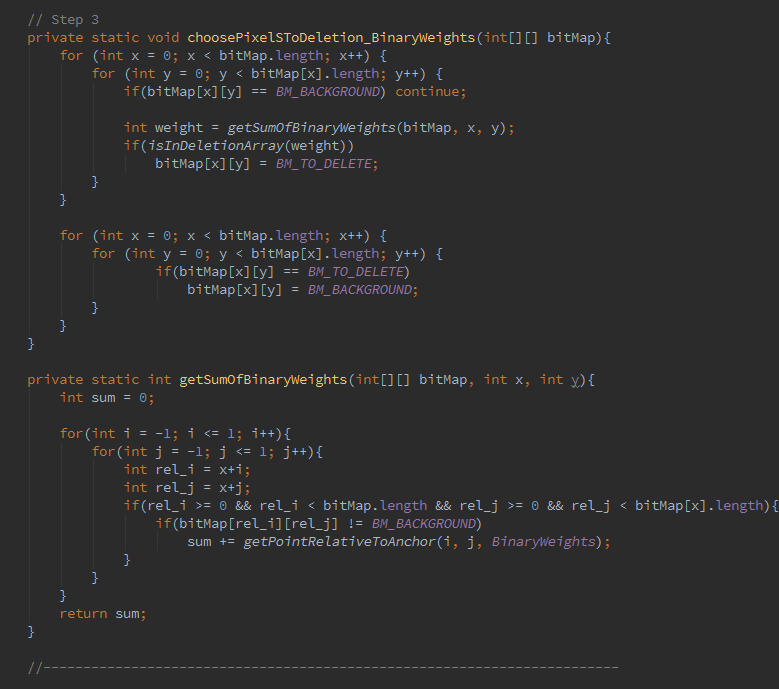
\includegraphics[width=0.9\linewidth]{res/kmm/binary_weights.png}

\caption{Choosing Pixels to Delete}
\label{fig:kmm_binary_weights}
\end{figure}


%%%%
%
% connectivity_main
%
%%%%
\begin{figure}[H]
\centering

  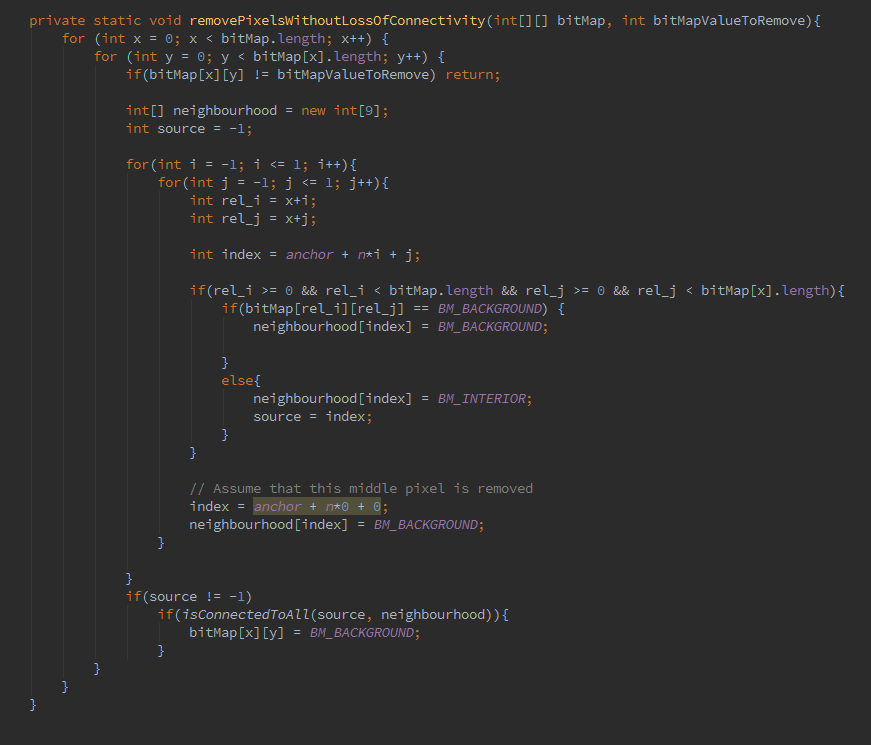
\includegraphics[width=0.9\linewidth]{res/kmm/connectivity_main.png}

\caption{Removing Pixels without loss of connectivity: Main loop}
\label{fig:kmm_conn_main}
\end{figure}



%%%%
%
% connectivity_isConnected
%
%%%%
\begin{figure}[H]
\centering

  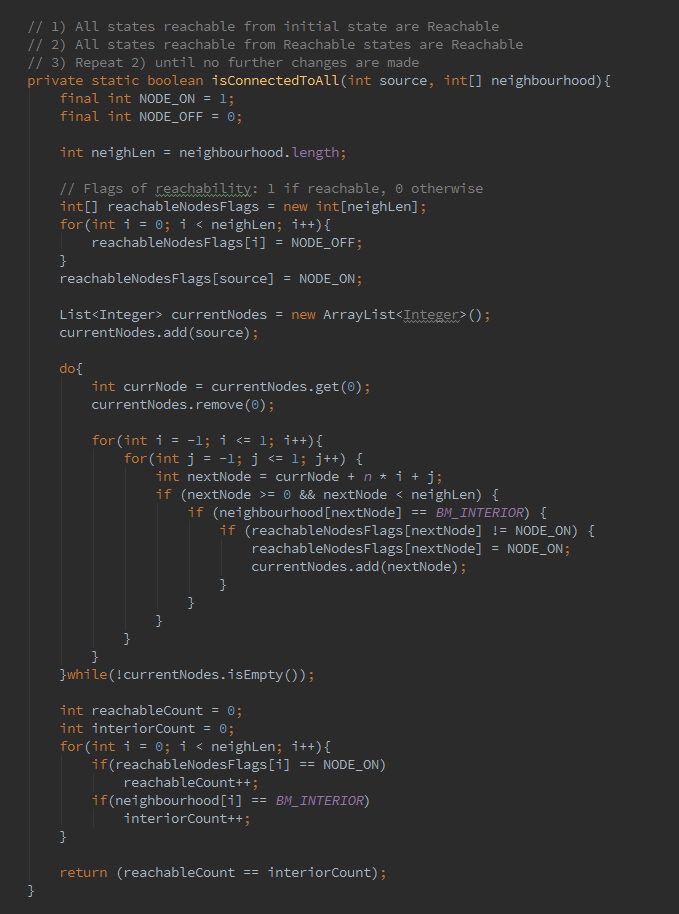
\includegraphics[width=0.9\linewidth]{res/kmm/connectivity_isConnected.png}

\caption{Finding if given sub neighbourhood is connected}
\label{fig:kmm_conn_is_conn}
\end{figure}

%%%%
%
% Utility
%
%%%%
\begin{figure}[H]
\centering

  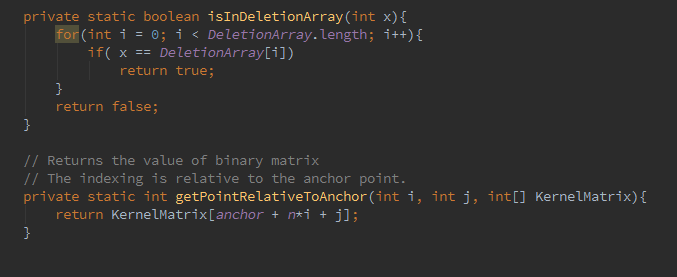
\includegraphics[width=0.9\linewidth]{res/kmm/util.png}

\caption{Utility Methods}
\label{fig:kmm_util}
\end{figure}

%----------------------------------------------------------------------------------------
\section{K3M}

\subsection{Algorithm}

Input to K3M is again a binary image where interior pixels (black) are coded in the Bit Map with value 1 and background pixels (white) are 0
A single iteration of K3M consists of 7 phases. The algorithm iterates until no further modifications of the input image is done. Each phase decides which pixel to be deleted based on a specific to this phase Deletion Array. The last phase of the algorithm is supposed to create a 1-pixel width skeleton. 

Let us consider the 7 phases of a single iteration. Firstly, defined a neighbourhood of a given Pixel as a 8-point neighbourhood which defines neighbours in the local area of the Pixel. Border pixels are pixels that stick in some way to the background. The border pixels are to be decided whether they should be removed or not. The Thinning decision is based on a 8-point neighbourhood template which defines a weight of the corresponding pixels in the neighbourhood. Phase 0 chooses the border pixels which then are potentially deleted in Phases 1 through 5.
The neighbourhood Bit Matrix looks as follows:

\[
N =
\begin{bmatrix}
	128 & 1  & 2 \\
	64  & 0  & 4 \\
	32  & 16 & 8
\end{bmatrix}
\]

The weight of the neighbourhood is calculated as follows:
\begin{center}
$w(x,y) = \sum^{1}_{i=-1} \sum^{1}_{j=-1} N(i+1,j+1)*I(x+i, y+j)$
\end{center}
Where I is the input image and N is the Bit Matrix.

Each Phase contains its own Look Up table. The Look Up table for Phase 0 is used to determine the border pixels. Phases 1 through 5 determine whether these border pixels should be removed based on their own Look Up tables.

Now the flow of Phase 0 is presented
\begin{enumerate}
	\item For each Pixel in the input image, do:
	\begin{enumerate}
		\item Let $(x,y)$ be the coordinates of tested Pixel
		\item Calculate Neighbourhood weight $w(x,y)$
		\item If the weight $w(x,y)$ is contained in the Look Up table $A_0$ then add the tested Pixel to border pixels
	\end{enumerate}	
\end{enumerate}

The Phases $i$ for $i = 1,2,3,4,5$ look as follows:
\begin{enumerate}
	\item For each Pixel in the border pixels, do:
	\begin{enumerate}
		\item Let $(x,y)$ be the coordinates of tested Pixel
		\item Calculate Neighbourhood weight $w(x,y)$
		\item If the weight $w(x,y)$ is contained in the Look Up table $A_i$ then set the tested Pixel to background color.
	\end{enumerate}	
\end{enumerate}

The Look Up tables for each Phase:
\begin{enumerate}
	\item Phase 0: $A_0$ - Marking borders
	\item Phase 1: $A_1$ - Deleting pixels having 3 sticking neighbours
	\item Phase 2: $A_2$ - Deleting pixels having 3 or 4 sticking neighbours
	\item Phase 3: $A_3$ - Deleting pixels having 3, 4 or 5 sticking neighbours
	\item Phase 4: $A_4$ - Deleting pixels having 3, 4, 5 or 6 sticking neighbours
	\item Phase 5: $A_5$ - Deleting pixels having 3, 4, 5, 6 or 7 sticking neighbours
	\item Phase 6: $A_6$ - Used for thinning the one-pixel width skeleton.
				
\end{enumerate}

Finally the flow of entire K3M algorithm looks as follows.
\begin{enumerate}
	\item For input binary image, iterate through Phases $1,2,3,4,5$
	\item Repeat iterations until no further modification to image have been computed.
	\item Compute the 1-pixel width phase.
\end{enumerate}


%----------------------------------------------------------------------------------------
\section{Comparison}
KMM used only one Look Up table where K3M uses plenty of them through out all of its phases. This leads to better quality results in the modified image.
Both K3M and KMM produce a one-pixel wide skeletons but K3M leads to better angle preservation.

Both K3M and KMM are sequential and iterative algorithms which defines their high computational complexities.


\end{document}